\chapter{Long-read Sequencing}\label{ch: long_read_sequencing}

This chapter provides a detailed background into the lab workflow and bioinformatics pipeline used to generate and analyse data from Pacific Bioscience's SMRT Sequencing (notably, Iso-Seq) and Oxford Nanopore Technology's nanopore cDNA sequencing. 

\section{Pacific Biosciences: Isoform Sequencing}
\label{sec:pb_isoform_sequencing}

\subsection{Introduction}
Successful DNA polymerisation requires a high concentration of nucleotides for DNA polymerase processivity and accuracy. However, mimicking this in DNA sequencing results in a high background noise level, and subsequently, reduces the sensitivity to detect base incorporation and fluorophore emission. Historically, second-generation sequencing technologies such as Illumina RNA-Seq have circumvented this issue by the step-wise addition, scan and wash of each set of labelled nucleotides, though at the expense of read lengths (discussed in \cref{rnaseq_intro}). 

In 2013, PacBio pioneered the development of third generation long-read sequencing with the capability to generate substantially longer reads (reviewed in \cref{tab: longread_isoseqstudies}), due to its ability to mimic the natural, uninterrupted, processive DNA synthesis through three important innovations \cite{Eid2009}: 
\begin{enumerate}
	\item The creation of a circular template, SMRTbell, which is enclosed with hairpin adapters at the ends of the insert, allowing uninterrupted DNA polymerisation \cite{Travers2010} (\cref{fig:Mechanism}\textbf{a}).
	\item Sequencing each polymerase-bound SMRTbell at the bottom of a nanometre-wide well (zero-mode-waveguide - ZMW\nomenclature{ZMW}{Zero-Mode-Waveguide})\cite{Levene2003}. The nanoscale size of the ZMWs and reduced volume allow sensitive detection of a single nucleotide incorporation event against the high background of labelled nucleotides, thereby achieving a high-signal-to-noise ratio (\cref{fig:Mechanism}\textbf{b}). PacBio currently offers two sequencers, which primarily differs in the number of ZMWs that can be sequenced: Sequel I and Sequel II with 1M and 8M ZMWs, respectively.   
	\item The addition of phospholinked nucleotides, each labelled with a different colour fluorophore corresponding to the four different bases (A, C, G and T), which allows for natural and processive DNA synthesis\cite{Mccarthy2010} (\cref{fig:Mechanism}\textbf{c}). 
\end{enumerate}

\vspace{1cm}
\subsubsection{Mechanism}
Due to the circular nature of the SMRTbell template, the polymerase is able to continually read through the insert in an interrupted fashion multiple times (or "passes"), resulting in a continuous read (known as polymerase read) (\cref{fig:Mechanism}\textbf{a}). By removing the hairpin-adapters that delineate the repeated insert sequence, this polymerase read is resolved to multiple reads (known as subreads), which are then merged to yield one high-quality and highly-accurate consensus read (known as Circular Consensus Sequence - CCS\nomenclature{CCS}{Circular Consensus Sequence}) (\cref{fig:Mechanism}\textbf{a}). The generation of these CCS reads can dramatically increase the read accuracy from 85\% (raw subreads) to 99\%, which is proportional to the number of "passes" and is dependent on the polymerase lifetime and insert length\cite{Travers2010}. 

Unlike RNA-Seq short reads, PacBio Iso-Seq reads are not of a set length, but a range of lengths that is reflective of the library size and dependent on polymerase activity\cite{Ardui2018,Rhoads2015}. Previous chemistries preferentially sequenced molecules of a certain length due to biased loading of SMRTbell templates - Diffusion Loading favoured shorter molecules\cite{Loomis2013} whereas Magbead Loading allowed proportional loading to the concentration rather than by length, but prevented sequencing of molecules <1kb (discussed in \cref{section:ch2_polbinding_loading}). However, recent improvements in both technology and chemistry have alleviated this sequencing read bias, eliminating the need for fractionating the library by length prior to sequencing (size selection) and resulting the Magbead loading method obsolete \cite{Oikonomopoulos2020}.

\begin{figure}[!h]
	\centering
	\includegraphics[page=14,trim={0 5cm 0 0 },clip, scale = 0.7]{Figures/ProjectDevelopment_Figures.pdf}
	\captionsetup{width=0.95\textwidth}
	\caption[Pacific Bioscience's Single Molecule Real-time Sequencing]%
	{\textbf{Pacific Bioscience's Single Molecule Real-time Sequencing (SMRT)}: PacBio's SMRT technology is able to generate long reads >10kb by \textbf{a)} enclosing the cDNA fragment of interest within a circular template (SMRTbell) to allow uninterrupted DNA polymerisation,  followed by the \textbf{b)} sequencing of each SMRTbell with a bound polymerase at the bottom of ZMWs, enabling sensitive detection of polymerisation at nucleotide level from \textbf{c)} addition of phospholinked nucleotides with differently labelled fluorophore. ZWW - Zero-Mode-Waveguide}
	\label{fig:Mechanism}
\end{figure}


\subsection{Library Preparation}
\label{chap:isoseq_labpipeline}
This section describes the lab workflow for PacBio Iso-Seq library preparation, which was applied in the long-read sequencing experiments in \textbf{Chapters 4,6} and \textbf{7}. Methods pertaining to sample preparation, cDNA synthesis and amplification can be found in \cref{ch: general methodology}.

The complete Iso-Seq lab workflow, as outlined in \cref{fig:isoseq_wholelab_protocol}, involved three main steps: i) converting RNA to full-length cDNA using the Clontech SMARTer PCR cDNA synthesis kit (described in \cref{section:ch2_cDNA_synthesis_explanation}), ii) amplification and purification of double-stranded cDNA, and (described in \cref{section:ch2_PCR_explanation}, \cref{section:ch2_AMPure_explanation}) iii) performing SMRTbell library preparation. The Iso-Seq lab workflow for the targeted profiling of the transcriptome, outlined in \cref{fig:isoseq_targetedlab_protocol} and for experiments in \textbf{Chapters 4} and \textbf{7}, involved an additional step of target gene enrichment after cDNA amplification and before SMRTbell library preparation, and the usage of barcode sequences in cDNA synthesis to allow sample multiplexing.

\begingroup
\parindent=0em
\etocsettocstyle{\rule{\linewidth}{\tocrulewidth}\vskip0.5\baselineskip}{\rule{\linewidth}{\tocrulewidth}}
\etocsetnexttocdepth{5}
\localtableofcontents 
\endgroup

\begin{figure}[htp]
	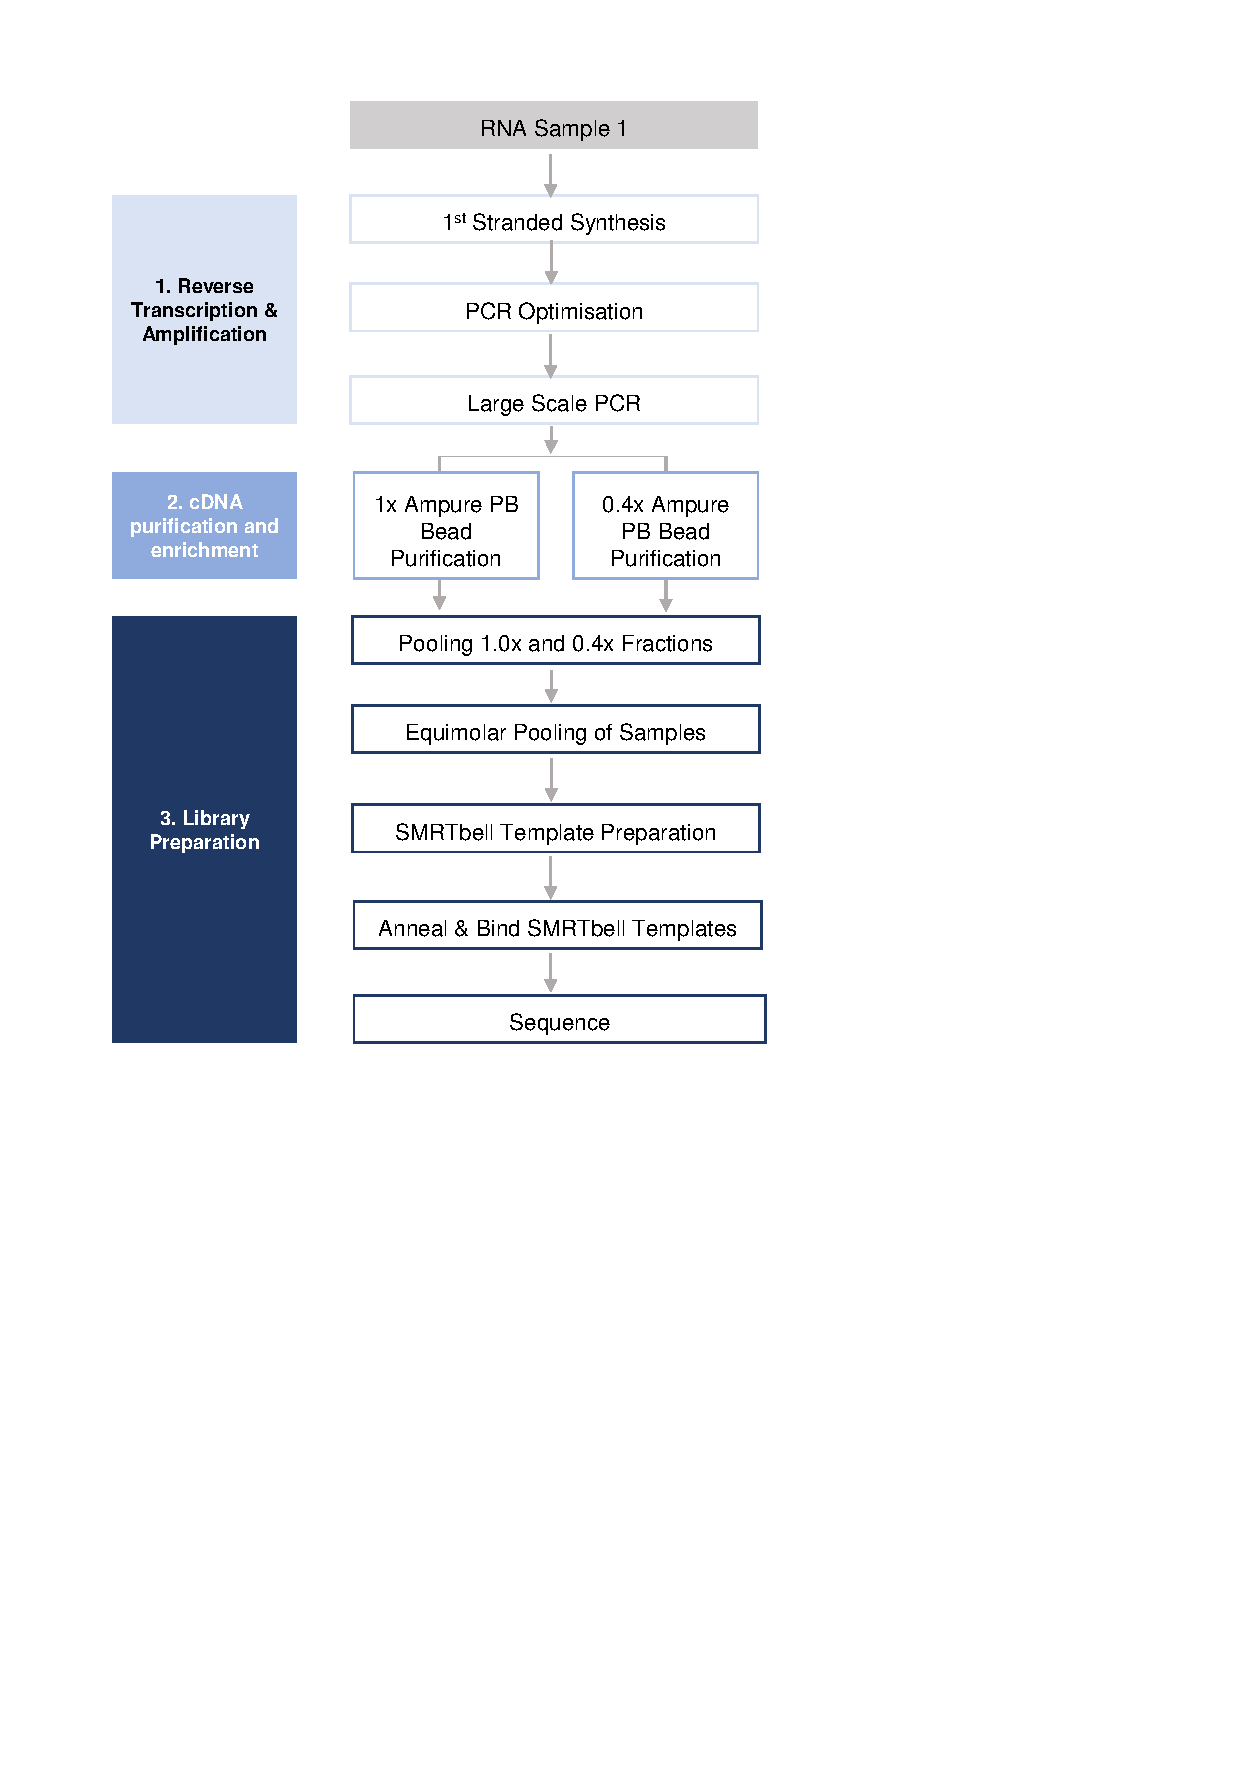
\includegraphics[page=1,trim={0 12cm 5cm 1cm},clip,scale = 1]{Figures/ProjectDevelopment_Figures.pdf}
	\captionsetup{width=0.95\textwidth}
	\caption[Iso-Seq Lab workflow used for global profiling of the transcriptome]%
	{\textbf{An overview of the lab Iso-Seq workflow for global profiling of the transcriptome}. The lab workflow, as adapted from official Iso-Seq protocol, involves three main steps: 1) reverse transcription and amplification of cDNA (\cref{section:ch2_cDNA_synthesis_explanation}), 2) cDNA purification with AMPure beads (\cref{section:ch2_AMPure_explanation}) and 3) library preparation involving ligation of SMRT bell templates, and binding of the primer and polymerase (\cref{section:ch2_smrtbelltemplate_explanation}). Due to the usage of newer chemistries, size selection was not performed.}
	\label{fig:isoseq_wholelab_protocol}
\end{figure}

\begin{figure}[]
	\begin{center}
		\includegraphics[page=2,trim={1cm 12cm 1cm 1cm},clip,scale = 0.8]{Figures/ProjectDevelopment_Figures.pdf}
	\end{center}
	\captionsetup{width=0.95\textwidth}
	\caption[Iso-Seq Lab workflow used for targeted profiling of the transcriptome]%
	{\textbf{An overview of the lab Iso-Seq pipeline used for targeted transcriptome profiling}. The lab workflow for targeted profiling of the transcriptome follows all the steps in the Iso-Seq lab workflow for global transcriptome profiling (depicted in Figure \ref{fig:isoseq_wholelab_protocol}), with the addition of target gene capture step (Boxed orange, \cref{section:ch2_targetcapture_explanation}) and the use of barcode sequences in cDNA synthesis (Boxed green and denoted here as Barcode 1 and Barcode n) to allow sample multiplexing (denoted here as Sample n). The list of barcodes can be found in \cref{tab:barcode_primers}}
	\label{fig:isoseq_targetedlab_protocol}
\end{figure}


\subsubsection{PCR optimisation and DNA Amplification}\label{ch: pcr_optimisation}
After cDNA synthesis, cDNA products were amplified using PCR to generate sufficient material for sequencing. To minimise PCR bias resulting in under or over representation of the different cDNA library size, the optimum number of PCR cycles for amplification was determined with PrimeSTAR GXL DNA Polymerase (Clontech) (\cref{fig:pcr_optimisation_gel_eg}). This involved collecting 5$\mu$L PCR aliquots every two cycles (cycles 10, 12, 14, 16, 18, 20) followed by visualisation of cDNA products on a 1.5\% Agarose gel with ethidium bromide. Large scale PCR amplification was then subsequently performed using the optimum number of cycles.  

\begin{figure}[htp]
	\begin{center}
		\includegraphics[page=13,trim={1cm 24cm 10cm 1cm},clip,scale = 0.9]{Figures/ProjectDevelopment_Figures.pdf}
	\end{center}
	\captionsetup{width=0.95\textwidth}
	\caption[Example of an Agarose gel for determining optimum number of PCR cycles for amplification]%
	{\textbf{PCR optimisation is required to determine optimum number of cycles}. Shown is an agarose gel of Human Brain Total RNA after first strand cDNA synthesis and PCR amplification through cycles 8 to 18, with PCR aliquots collected during respective cycles. In this example, 10 cycles were determined to be the optimum number for large-scale amplification. While smear distribution from 8 and 10 cycles look similar, 10 cycles show a slightly stronger smear, thereby generating more material for downstream pooling. Cycles above 12 show signs of over-amplification which will result in biased sequencing representation. Figure and legend are adapted from Iso-Seq protocol}
	\label{fig:pcr_optimisation_gel_eg}
\end{figure}


\subsubsection{AMPure Bead Purification} 
After large scale amplification, the resulting PCR products were divided into two fractions for purification with either 0.4X or 1X AMPure PB beads (PacBio). DNA purification with 0.4X AMPure beads was essential to ensure enrichment of longer fragments for sequencing (as described in \cref{section:ch2_AMPure_explanation}). Quantification and size distribution of each fraction was then determined using Qubit DNA High sensitivity assay (Invitrogen) and Bioanalyzer assays on the 2100 Bioanalyzer (Agilent) for calculating the molarity of the two fractions (using the \textbf{Equation \ref{eqn:isoseq_library_molarity}}). Equal molar quantities of the two fractions were then pooled for library construction with the SMRTbell Template Prep Kit v1.0 (PacBio). 

\begin{equation}
	\label{eqn:isoseq_library_molarity}
	\frac{concentration(\frac{ng}{ul})\times 10^6}{660(\frac{g}{mol}) \times average\:library\:size\:in\:bp\mbox{*}} = concentration\;in\; nM
\end{equation}
* the average library size was determined by the start and end point of the smear

\subsubsection{Target Capture using IDT Probes} 
\label{section:ch2_targetcapture_explanation} 
Targeted profiling of the transcriptome was performed as part of long-read sequencing experiments in \textbf{Chapters 6} and \textbf{7}. Equal molar quantities of uniquely-barcoded samples were pooled for target enrichment, which was performed using a hybridisation capture approach (IDT); regions of interest within the library (amplified and purified cDNA) were captured with pre-designed, complementary 5’ biotinylated DNA 120nt-long oligonucleotide baits (hereby referred as probes) (depicted in \cref{fig:isoseq_targetcapture}\textbf{a}). After hybridisation of probes, magnetic streptavidin beads were used to separate the hybridised library fragments, which were then amplified using Takara Hot-Start polymerase followed by AMPure bead purification (outlined in \cref{fig:isoseq_targetcapture}\textbf{b}). After assessing the quality and quantity of the target cDNA  Qubit DNA High sensitivity assay (Invitrogen) and Bioanalyzer assays on the 2100 Bioanalyzer (Agilent), SMRTbell library preparation was proceeded according to manufacturer's protocol.  

%*Modifications to the protocol: waiting times at room temperature during hybridisation, lid heat temperatures, method of washing beads at room temperature; all modifications are incorporated from official IDT protocol, post amplification clean-up for consistency  

\myparagraph{Probe Design}
Probes were designed to a panel of 20 AD-associated genes: \textit{Abca7, Abca1, Ank1, Apoe, App, Bin1, Cd33, Clu, Fus, Fyn, Mapt, Picalm, Ptk2b, Rhbdf2, Snca, Sorl1, Tardbp, Trem2, Trpa1, Vgf}. Two separate pools of equal molar probes were designed against the mouse (GRCm28/mm10) and human genome (GRCh37/hg19). While IDT provided a pre-designed set of probes to the exons of target genes (depicted in \cref{fig:target_probes_eg}\textbf{a}), the majority of exons were unnecessarily covered by contiguous probes, which induces off-target binding and additional costs. Given that previous targeted sequencing studies using the same hybridisation capture have achieved successful enrichment and sequencing with a few unique probes to the exonic region\cite{Sheynkman2020}, I manually assessed the list of probes for each target gene using the following criteria:
\begin{itemize}
	\item All of the exons must be covered by at least one probe
	\item Probes should be spaced 300-500bp within each exon (equivalent to 0.2x – 0.3x tiling density) 
	\item Probes with the highest GC content (40-65\% GC content) and lowest number of blast hits were selected from the contiguous cluster 
	\item Any probes covering the intronic regions were removed
\end{itemize}
Examples of the probes provided by IDT and the final curated sets are illustrated in  \cref{fig:target_probes_eg}\textbf{b - d}. The final number of human and mouse probes are provided in the Methods section of the respective Chapters.

\begin{figure}[!h]
	\begin{center}
		\includegraphics[page=12,trim={0cm 6cm 0cm 1cm},clip,scale = 0.70]{Figures/ProjectDevelopment_Figures.pdf}
	\end{center}
	\captionsetup{width=0.95\textwidth}
	\caption[Lab workflow for hybridisation capture of cDNA for targeted transcriptome profiling]%
	{\textbf{Lab workflow for hybridisation capture of cDNA for targeted transcriptome profiling.} An overview of the lab workflow of the target gene enrichment involving hybridisation of cDNA with probes and blockers (polyT oligonucleotide, cDNA synthesis primers), followed by capture with streptavidin beads. The addition of blockers prevent non-specific binding, and subsequently increases capture rate and target gene sequencing coverage}
	\label{fig:isoseq_targetcapture}
\end{figure}

\begin{landscape}
	\begin{figure}[ht]
		\begin{center}
			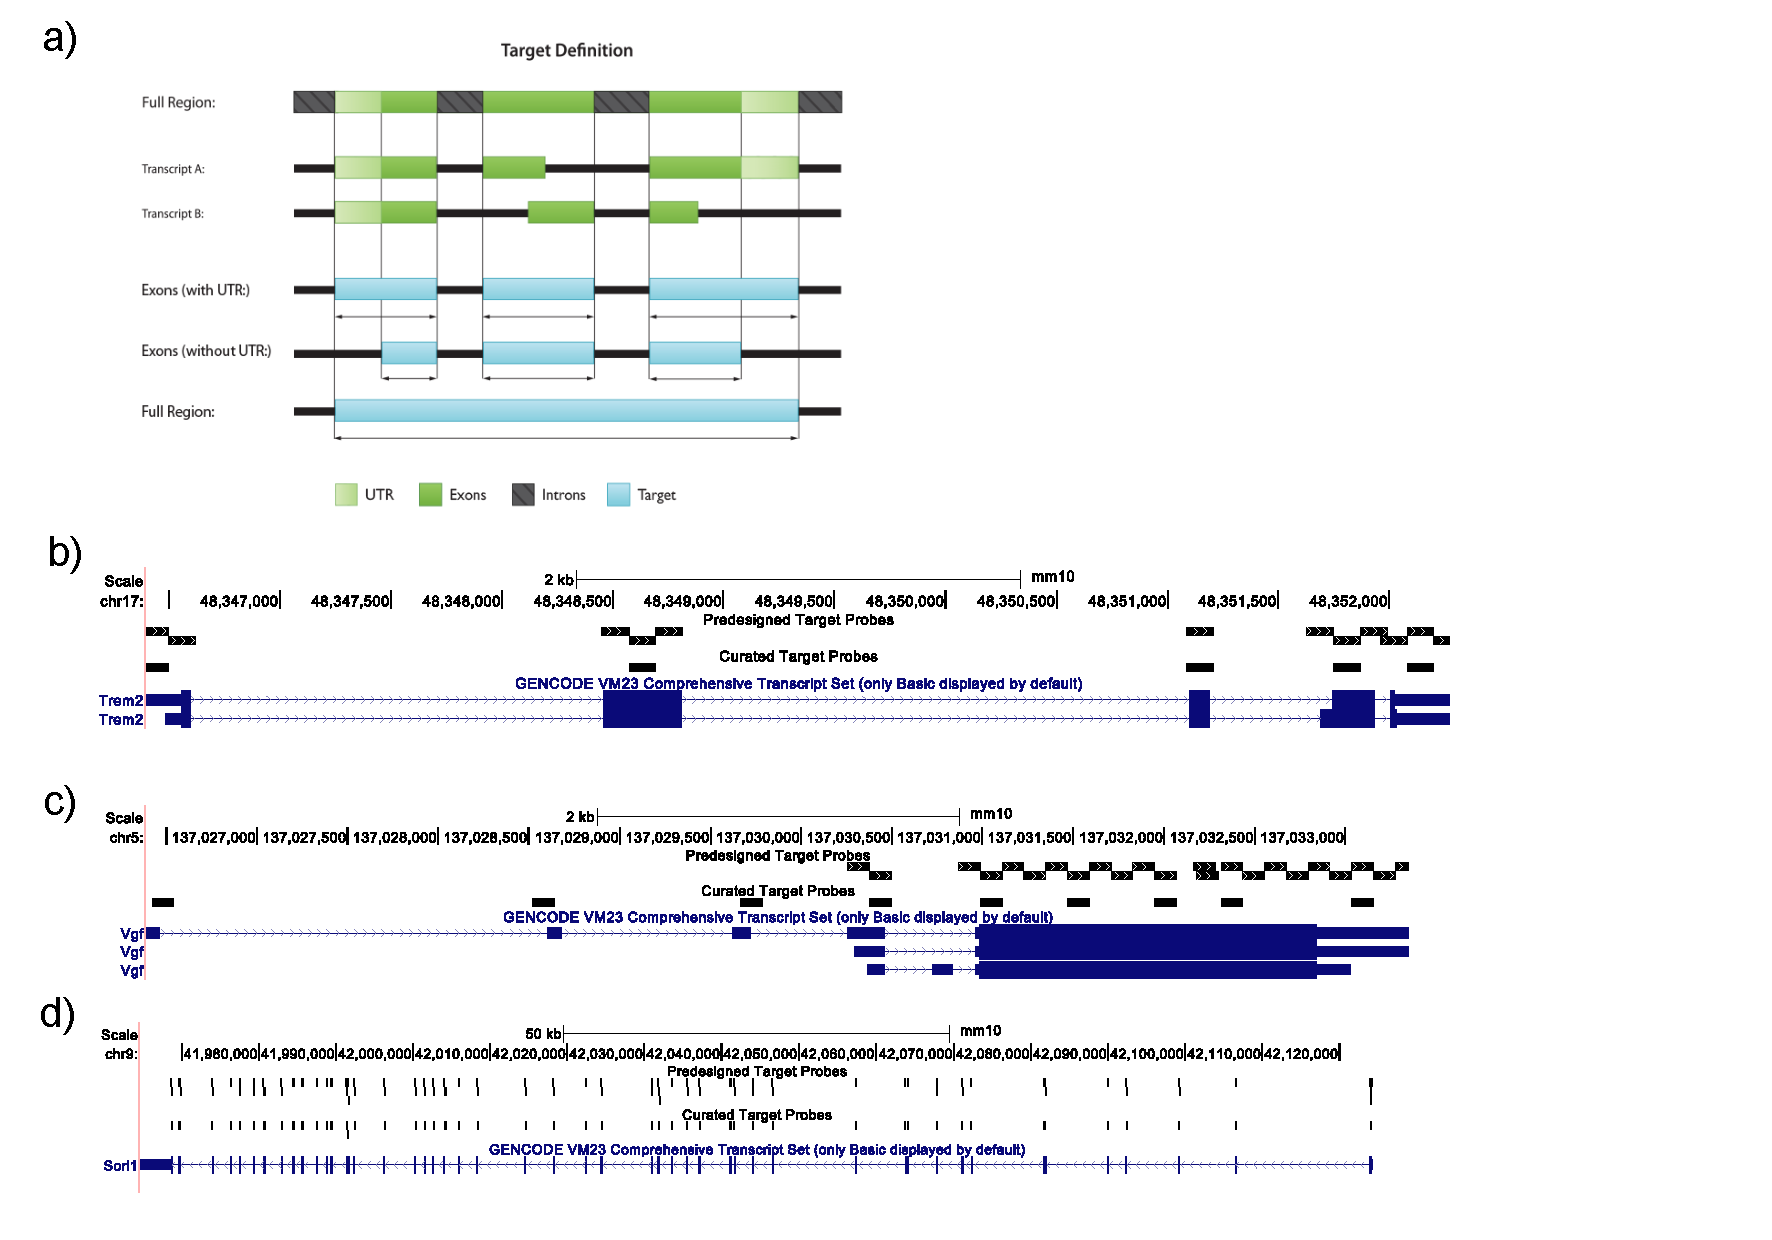
\includegraphics[page=1,trim={0cm 2cm 0cm 0cm},clip,scale = 0.70]{Figures/TargetProbes_Visualisation.pdf}
		\end{center}
		\captionsetup{width=1.5\textwidth}
		\caption[Manual curation of probes designed to 20 AD-associated target genes]%
		{\textbf{Manual curation of probes designed to 20 AD-associated target genes.} \textbf{a)} Pre-designed set of probes were provided to "Exons (without UTR)" of target genes. However, exons were unnecessarily covered by contiguous probes which not only induces additional costs but also off-target binding (referred in figure as Pre-designed Target Probes). Manual curation was therefore needed for each target gene (referred in figure as Curated Target Probes) to ensure that exons were covered with one probe for every 500bp. Shown in \textbf{b,c,d)} are UCSC genome browser tracks of pre-designed and curated probes to \textit{Trem2}, \textit{Vgf} and \textit{Sorl1} in the mouse genome (mm10).}
		\label{fig:target_probes_eg}
	\end{figure}
\end{landscape}

\subsubsection{Library Preparation, Primer Annealing \& Polymerase Binding}
\label{section:ch2_smrtbelltemplate_explanation} 
After pooling the two fractions for global transcriptome profiling or multiple samples for targeted sequencing at equal molar quantities, SMRTbell template preparation was performed with the SMRTbell Template Prep Kit v1.0 (PacBio). This first involved repairing DNA damage and polishing ends of fragments (\cref{fig:isoseq_labworkflow}, Step 1, 2), essential for the generation of high-quality library of closed, continuous and circular SMRTbell templates. Abasic sites were filled, thymine dimers resolved, and deaminated cytosine alkylated. 3’ overhangs were removed, whereas 5’ overhangs were filled-in by T4 DNA Polymerase and phosphorylated by T4 PNK for ligation of blunt hairpin adapters. Following 1x AMPure bead purification of repaired dsDNA, hairpin adapters were ligated to the blunt ends for 24hours (\cref{fig:isoseq_labworkflow}, Step 3). Any templates failing to ligate were removed with exonuclease III and VII (\cref{fig:isoseq_labworkflow}, Step 4). The repaired, ligated SMRTbell library was then purified with 2 rounds of 1x AMPure beads, and assessed for quality and quantity with Qubit DNA High sensitivity assay (Invitrogen) and Bioanalyzer 2100 before proceeding to primer annealing and polymerase binding (\cref{fig:isoseq_labworkflow}, Step 5, 6). Of note, the primer and polymerase to template ratio is key to successful loading of SMRTbell templates into ZMWs for sequencing, and is dependent on the final library molarity (as determined using \textbf{Equation \ref{eqn:isoseq_library_molarity}}). 


\subsubsection{Loading and Sequencing} 
\label{section:ch2_sequencing}
All Iso-Seq experiments in this thesis were performed on the PacBio Sequel 1M SMRT cell. Samples were processed using either the v3 chemistry (diffusion loading at 5pM, pre-extension 4 hours, Capture time 20 hours) or v2.1 chemistry (Magbead loading at 50pM with a 2 hour pre-extension and 10 hour capture). All the samples bar the first two were sequenced using Diffusion loading. As the name suggests, Diffusion Loading involves immobilising polymerase-bound SMRTbells to ZMW by diffusion, whereas Magbead loading involves immobilising SMRTbells using paramagnetic beads ("Magbeads") that roll across the ZMWs. Due to the different nature of loading, Diffusion loading preferentially loads shorter transcripts, whereas Magbead loading preferentially loads longer transcripts (>1b). For quality-control measure of loading and sequencing performance, a DNA Internal Control Complex (PacBio) is added to each library before sequencing, the amount of which is dependent on the final library molarity. Mimicking SMRTbell templates, this Internal Control is composed of a 1966bp-insert that has already been ligated with SMRTbell adapters and polymerase-bound.


\begin{figure}[!htp]
	\begin{center}
		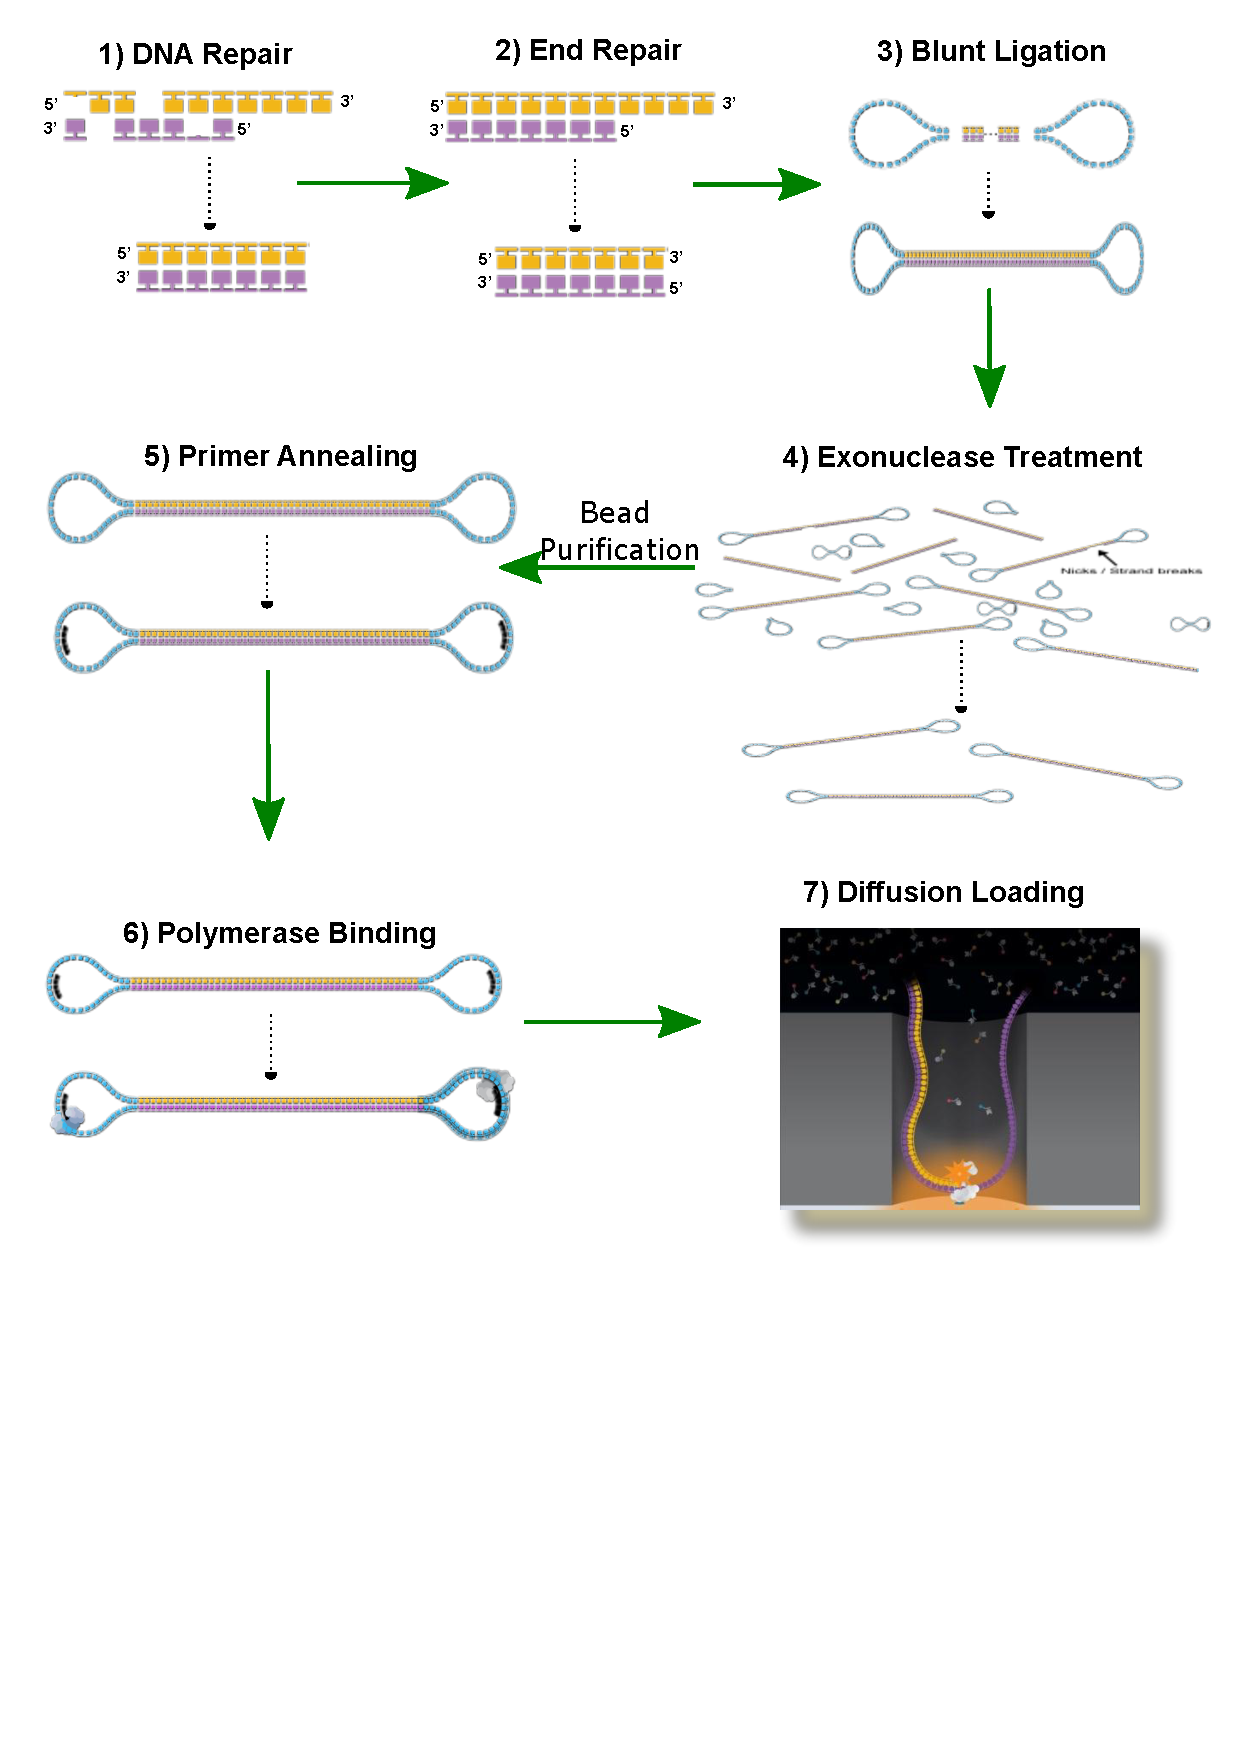
\includegraphics[page=1,trim={0cm 8cm 0cm 0cm},clip,scale = 0.70]{Figures/labwork_isoseq.pdf}
	\end{center}
	\captionsetup{width=0.95\textwidth,singlelinecheck=off}
	\caption[Lab workflow of Iso-Seq SMRT Bell Template Preparation, Primer Annealing \& Polymerase Binding]%
	{\textbf{Lab workflow of Iso-Seq SMRT Bell Template Preparation, Primer Annealing \& Polymerase Binding.} Shown is a flow diagram of the lab workflow of Iso-Seq library preparation for long-read sequencing on the Sequel:
		\begin{enumerate}
			\item Repair DNA Damages by repairing abasic sites and nicks, removing thymine dimers, oxidising guanines, deaminating cytosine; essential to ensure continuous sequence for uninterrupted polymerase processivity 
			\item Repair ends for blunt ligation with removal of 3' hangs and addition of 5' hangs by T4 DNA polymerase; essential for blunt ligation of SMRT bell adapters 
			\item Blunt Ligation by adding hairpin SMRT bell adapters to repaired ends
			\item Exonuclease treatment to remove incomplete SMRTbells with Exonuclease III and IV; essential to ensure sequencing of good library 
			\item Annealing of primer to both ends of the SMRT bell templates to initiate sequencing 
			\item Binding of polymerase to both ends of SMRT bell templates for efficient loading into ZMWs
			\item Immobilisation of polymerase-bound SMRTbells to ZMW by diffusion
			\\
		\end{enumerate} 
		Individual figures and legend are taken and adapted from "PacBio Sequel Library and Sequencing Preparation" presentation
	}
	\label{fig:isoseq_labworkflow}
\end{figure}

\clearpage
\subsection{Run Performance and Run Quality Metric}
Suboptimal PacBio sequencing performance could be due to various reasons from potential issues with the instrument and sequencing reagents to poor library preparation and incorrect loading. The performance of a sequencing run can be assessed by the performance of the DNA Internal Control and productivity metrics. 

\boldheader{DNA Internal Control} 
Sequencing metrics for the DNA Internal Control (described in \cref{section:ch2_sequencing}) is provided in several ways: i) the number of control reads, ii) the mean control polymerase read length iii) the proportion of sequence identity match between the control raw reads and the reference control (concordance). Short control read lengths and/or low control read counts are suggestive of issues with the PacBio instrument and consumables, while a low concordance value (<0.84) indicate overloading of SMRT cells. Conversely, normal control sequencing metrics in a run with overall low yield indicate sample-specific issues. The expected sequencing metrics from a correctly prepared control in a good sequencing run are documented in \cref{tab:control_Isoseqmetrics}. 

\vspace{1cm}
\begin{table}[!h]
	%\captionsetup{justification=raggedright,width=1.45\textwidth}
	\caption[Iso-Seq DNA Internal Control Sequencing Metrics]%
	{\textbf{Iso-Seq DNA Internal Control Sequencing Metrics.} Tabulated are the expected median values for the number of control reads (median count), the control polymerase read length (median length), and the identity match between control raw reads and reference sequence (median concordance). The expected values provided assume a sequencing run performed on the PacBio Sequel 1M SMRT cell with a 4hr pre-extension time and a 20hr capture time}
	\label{tab:control_Isoseqmetrics}
	
	\centering
	\begin{tabular}{@{}cccc@{}}
		\toprule
		Metrics         & Median Count (QR)     & Median Length (kb) (QR) & Median Concordance (QR) \\ \midrule
		Expected Values & 6900 (4,000 - 10,200) & 46.9 (41.5 – 52.5) & 0.862 (0.857 – 0.867)   \\ \bottomrule
	\end{tabular}
\end{table}


\boldheader{Productivity Metrics} 
Productivity or loading metrics is a measure of the number of ZMWs that generated a positive signal that is translated into useful sequencing data. Each ZMW is classified as either: 
\begin{itemize}
	\item P0 (Productivity 0): no active sequencing polymerase complex with no signal 
	\item P1 (Productivity 1): productive ZMWs with a high quality (HQ) region* within read 
	\item P2 (Productivity 2): detectable signal but no HQ region* detected, possibly due to overloading of multiple inserts with multiple polymerases
\end{itemize}
*HQ region is defined as a high quality sequence of >50bases. These metrics are also dependent on chemistry, pre-extension, and movie runtime.  

An optimal sequencing run is indicated by a run yield of 20-30Gb with \textasciitilde70\% of ZWMs in P1 (positive signal), and 20-30\% ZMWs in P0 (empty ZMWs). A low P0 (<20\%) indicate over-loading of polymerase-bound templates, resulting in shorter P1 polymerase reads and poor sequencing yield (noisy base-calling). Conversely, a high P0 (>40\%) from under-loading would generate fewer P1 reads and result in low sequencing yield. A combination of high P0, low P1 and high P2 loading profiles indicates presence of contaminants (possibly from poor AMPure bead purification) that is interfering with productive polymerase activity. A good balance between P0, P1 and P2 is therefore key to achieving a good sequencing run with high yield and high-quality, long P1 polymerase reads. Multiple titrations of loading concentrations can be trialled to determine the optimum loading concentration essential for reaching this balance. 

\clearpage
\subsection{Bioinformatics Pipeline} 
\label{section:isoseq_bioinformatics}
This section describes the bioinformatics pipeline for analysing Iso-Seq data generated on the PacBio Sequel I following Iso-Seq library preparation (\textbf{Chapters 4 - 7}). 

The bioinformatics pipeline, as depicted in \cref{fig:isoseq_bioinformatics_Pipeline}, involved three main steps: i) processing and filtering of raw reads into high-quality (HQ), full-length transcripts using \textit{IsoSeq3}, ii) alignment of HQ transcripts to the reference genome using \textit{Minimap2} and iii) collapse mapped transcripts to unique, annotated isoforms using \textit{Cupcake} and \textit{SQANTI}. Public annotations and short-read RNA-Seq data was used for validating Iso-Seq derived isoforms. While Iso-Seq raw data can be processed using the PacBio SMRT Link Suite, a web-based end-to-end user interface, we developed an end-to-end command line that allowed simultaneous processing of multiple samples (parallelisation) and included steps after raw read processing. The choice of parameters and packages was guided by a separate analysis on sequenced external RNA Spike-In controls (ERCC, described in \cref{section:ch2_ERCC_explanation}). 

\begingroup
\parindent=0em
\etocsettocstyle{\rule{\linewidth}{\tocrulewidth}\vskip0.5\baselineskip}{\rule{\linewidth}{\tocrulewidth}}
\etocsetnexttocdepth{5}
\localtableofcontents 
\endgroup


\begin{figure}[]
	\centering
	\vspace{20pt}
	\includegraphics[page=17,trim={0 4.5cm 0 0},clip,scale = 0.8]{Figures/ProjectDevelopment_Figures.pdf}
	\captionsetup{width=0.95\textwidth}
	\caption[PacBio Iso-Seq Bioinformatics Pipeline]%
	{\textbf{An overview of the PacBio Iso-Seq Bioinformatics Pipeline}: The bioinformatics pipeline involves three main steps: i) processing and filtering of raw reads into high-quality (HQ), full-length transcripts using \textit{IsoSeq3} (v3.2.2), ii) alignment of HQ transcripts to the reference genome using \textit{Minimap2} and iii) collapse mapped transcripts to unique, annotated isoforms using \textit{Cupcake} and \textit{SQANTI3}}
	\label{fig:isoseq_bioinformatics_Pipeline}
\end{figure}

\clearpage
\subsubsection{Processing of Iso-Seq raw reads}
\label{section: Isoseq_rawprocessing}
In response to a much higher experimental throughput of PacBio Sequel compared to RSII, the official PacBio bioinformatics package for processing long Iso-Seq reads (\textit{Iso-Seq3}) has been revised multiple times over the course of this research. Each subsequent version saw a reduction in runtime coupled with an improvement in sensitivity and specificity to recover transcripts and reduce artefacts. One of the greatest changes was eliminating the usage of non-full-length reads or RNA-Seq short-reads for error correction due to the high throughput and subsequent generation of high-quality, accurate Iso-Seq reads. 

Despite multiple major updates of the package, the core processing steps of \textit{Iso-Seq} have remained the same: i) CCS with the generation of CCS reads from each sequencing ZMW, ii) Classify with identification of full-length reads followed by cDNA primers and polyA tail removal and iii) Cluster with grouping of full-length reads derived from the same transcript. 

\boldheader{Generation of CCS reads with \textit{CCS}}
Raw Iso-Seq subreads from each “productive” ZMW were processed to generate one representative circular consensus read (\cref{fig:Mechanism}\textbf{a}) using \textit{CCS} (v5.0.0) with the following parameters: 
\begin{itemize}
	\item minimum number of full "passes" for a ZMW to be used. A full pass is defined by the presence of both SMRT adapters at both ends (default: 3 passes)
	\item minimum predicted read accuracy across all subreads (default: 99\%)
	\item minimum and maximum length of subreads to generate a CCS (default: minimum 10 bases, maximum 21000 bases)
	\item Quality of subreads predicted by the CCS model (default: Z-score of -3.5), and proportion of total subreads meeting the quality score (default: \textgreater 30\%)
\end{itemize}

%Across literature and PacBio scientific community, different parameter settings were recommended, particularly with \textit{number of full passes} and \textit{minimum base accuracy}, which had the greatest effect on the number of CCS reads generated for downstream analyses. Taking a subset of raw data from 10 randomised samples, a range of values across these two parameters were tested. CCS were then classified to full-length (FL, determined by the presence of 3'/5' primers and poly-A tail) and non-full-length (NFL) reads. 

\boldheader{Removal of primers and barcodes with \textit{Lima}}
After the successful generation of CCS reads, cDNA primers and barcodes (PacBio) were identified and removed using \textit{Lima} (v2.0.0) to generate full-length (FL) reads. Additional barcode sequences were only included for targeted sequencing experiments where sample multiplexing was removed. Sequences were oriented from 5’ to 3’ and any reads with unwanted combinations were removed. The proportion of FL reads (number of FL reads over the number of CCS reads) varied on the insert transcript size, but a library with a distribution of 1-3kB is estimated to generate 60-70\% FL reads.  

\boldheader{Trimming of poly(A) tails and concatemer removal with \textit{Refine}}
Full-length reads were further refined by the trimming of poly(A) tails (with a minimum length of 20 adenosine bases), and removal of artificial concatemers to generate full-length non-chimeric (FLNC) reads. Artificial concatemers are defined as cDNA sequences with internal runs of polyA and polyT sequences, generated from using insufficient amount of blunt adapters during library preparation. The occurrence of these artefacts should be low (<0.5\%) in a standard library preparation. The number of FLNC reads and FL reads should therefore be similar, whereas any significant loss of reads at this stage implicates SMRTbell library preparation issues.

\boldheader{Grouping of reads into transcripts with \textit{Cluster}}
Using an iterative isoform-clustering algorithm, two or more FLNC reads were considered to be the same transcript, if the reads: 
\begin{itemize}
	\item differed < 100bp on the 5’ end* 
	\item differed < 30bp on the 3’end 
	\item Did not contain internal gaps with > 10bp
\end{itemize}
* Greater leeway was given to the 5'end than the 3'end to account for 5' RNA degradation

A minimum of two FLNC reads was required for clustering with the longest read chosen as the representative transcript, and any unique FLNC read failing to cluster were discarded. Transcripts generated from the \textit{Iso-Seq Cluster} were therefore high quality (HQ) with a consensus accuracy $\geq$99\% and $\geq$ 2 FLNC read support. 

\begin{figure}[htp]
	\centering
	\includegraphics[page=18,trim={0 7cm 0 0},clip,scale = 0.8]{Figures/ProjectDevelopment_Figures.pdf}
	\captionsetup{width=0.95\textwidth}
	\caption[PacBio Iso-Seq Bioinformatics Pipeline]%
	{\textbf{An overview of the PacBio Iso-Seq Bioinformatics Pipeline}: So in summary, each productive ZMW generates one polymerase read, which is collapsed to give a circular consensus sequence (CCS) assuming the requirements were met. CCS were then trimmed and processed for primer and poly-A sequence removal to generate full-length non-chimeric (FLNC) reads, which were clustered if they were thought to be derived from the same isoform. The number of associated full-length (FL) reads of each isoform therefore represents the number of ZMWs that sequenced the isoform of interest, and can infer abundance of mRNA isoform. However, Iso-Seq is only semi-quantitative due to preferential loading and sequencing bias of shorter fragments. It is worthy to note that all the steps up to now have been processed without a reference genome or transcriptome.}
	\label{fig:isoseq3_tool}
\end{figure}

\newpage
\subsubsection{Alignment to reference genome} 
%check section content
HQ-transcripts generated from \textit{IsoSeq} package were then aligned to the reference genome using \textit{Minimap2}, a splice-aware aligner that is faster, more precise and accurate than other mainstream mappers such as \textit{GMAP, BWA-MEM} \cite{SimirKriZanoviC2018,Tang2020}. Under the following recommended parameters, "-ax splice -uf --secondary=no -C5 -O6,24 -B4”,  \textit{Minimap2} prioritises the known canonical junctions (GT[A/G]…[C/T]AG) over non-canonical splice junctions (GT[C/T]…[A/G]AG), assumes that read orientation is unknown and therefore performs two rounds of alignment to infer orientation with the forward transcript strand for alignment, which slightly improves accuracy. 

\subsubsection{Further transcript collapse to isoforms using \textit{Cupcake}}
Aligned HQ-transcripts were filtered and further collapsed to unique, full-length, high-quality isoforms using \textit{Cupcake} (collapse\_isoforms\_by\_sam.py script) with the following parameters  “-c 0.85 -i 0.95 --dun-merge-5-shorter” to reduce redundancy - i.e. ensure that reads were correctly clustered in \textit{IsoSeq3 Cluster}. HQ transcripts with 85\% coverage and 95\% identity to the reference genome were removed. The number of associated FL reads associated with each isoform was obtained as proxy of isoform abundance using the \textit{Cupcake} (get\_abundance\_post\_collapse.py script) and custom script. 

\subsubsection{Transcriptome annotation with \textit{SQANTI}}
\label{section: sqanti_annotations}
Isoforms were characterised using SQANTI\cite{Tardaguila2018} which i) performs a reference-based correction of sequences, ii) classifies isoforms based on splice junctions, ii) annotates the transcriptome with user-defined public annotations and matched RNA-Seq data, and iv) filters out technical artefacts. 

\boldheader{Isoform classification by splice junctions}
Isoforms were classified as either annotating to known genes as a known or novel isoform, or to novel genes not currently annotated in existing genome annotations. Classifications were based on splice junctions, with an isoform classified as Full Splice Match (FSM) if it aligned with the reference genome with the same splice junctions and same exonic structure, Incomplete Splice Match (ISM) if it contained fewer 5’ exons than reference genome, Novel in Catalogue (NIC) if contained a different exonic structure with a combination of known donor or acceptor sites, or Novel Not in Catalogue (NNC) if it contained at least one novel donor or acceptor site. Depictions of RNA isoform classifications can be found in \cref{fig:sqanti_cate}. Splice junctions were defined by the two pairs of dinucleotides present at the intron boundary, and all GT-AG, GC-AG and AT-AC pairs were considered canonical, and all other possible combinations as non-canonical. 

Isoforms were also classified as protein-coding by the presence of open reading frames (ORF), which were predicted using the GMST algorithm, considering only the direct strand of the cDNA and AUGs as the initial codon. For incomplete isoforms (ISMs) with shortened 5' end, ORF was predicted from the first in-frame methionine, resulting in shortened N terminus. An isoform was predicted to undergo nonsense mediated decay if there is a predicted ORF and the coding sequence (CDS) ends at least 50bp from the last junction. 

\boldheader{Public annotations and matched RNA-Seq data}
Multiple public annotations were supplied into \textit{SQANTI} for deeper characterisation of the transcriptome. These annotations included:
\begin{itemize}
	\item Cap Analysis of Gene Expression (CAGE) Peak from FANTOM5 dataset, which map transcripts, transcription factors, transcriptional promoters and enhancers
	\item Intropolis junction bed file\cite{Nellore2016} from a comprehensive human RNA-Seq dataset
	\item Human and mouse poly(A) motifs provided by \textit{SQANTI}	 
\end{itemize}

Matched RNA-Seq data was also supplied to \textit{SQANTI} in two forms: i) after alignment to reference genome using \textit{STAR} for junction support and ii) alignment to \textit{Cupcake}-derived Iso-Seq transcripts using \textit{Kallisto} (v0.46.0)\cite{Bray2016} for RNA-Seq expression.  

\begin{landscape}
	\begin{figure}[h]
		\centering
		\includegraphics[page=3,trim={0 3cm 0 0},clip,scale = 0.8]{Figures/ProjectDevelopment_Figures_Landscape}
		\captionsetup{width=1.5\textwidth}
		\caption[Isoform Classifications by SQANTI]%
		{\textbf{Isoform Classifications by SQANTI}. Isoforms were classified by SQANTI as novel or known, and annotated to novel or known genes based on splice junctions}
		\label{fig:sqanti_cate}
	\end{figure}
\end{landscape}

\boldheader{Further filtering for technical artefacts}
\textit{SQANTI Filter} was used to filter the curated transcriptome from any technical artefacts that were generated during library preparation: i) RT template switching which occurs when RT transits within or across DNA templates without terminating cDNA synthesis if the original DNA template harbours two or more direct repeats\cite{Cocquet2006} (\cref{fig:lib_prep_artifacts}), and ii) off-priming when oligo(dT) primer binds to other internal homo-polymeric adenines (A) regions that can be located within cDNA template \cite{Conesa2016} (\cref{fig:lib_prep_artifacts}). These events can generate chimeric or short incomplete and truncated cDNA, that can be misinterpreted as isoforms generated from non-canonical splicing \cite{Houseley2010}. Using \textit{SQANTI}, we were able to identify RT-switch events by searching for direct repeats (given that RT switching is homology dependent) and intra-priming events by filtering out any isoform which has < 60\% of adenosines (A) within the 20 nucleotide window in the genome downstream of the isoform transcription termination site - the lower the percentage of genomic As after the TSS, the lower the chance of poly(A) tail being present and  higher the likelihood of off-priming. 

\begin{figure}[h]
	\begin{center}
		\includegraphics[page=4,trim={2cm 21cm 0 1cm},clip, scale = 1]{Figures/ProjectDevelopment_Figures.pdf}
	\end{center}
	\captionsetup{width=0.95\textwidth}
	\caption[Technical artefacts generated during library preparation and identified in SQANTI]%
	{\textbf{SQANTI identifies technical artefacts that were generated during first-strand cDNA synthesis a)}: Schematic diagram of reverse transcription template switching, taken from Cocquet et al.(2006) \cite{Cocquet2006}. The black and blue line represent the original cDNA and synthesising cDNA from RT respectively, the black box represent the direct repeats and the light grey sphere represent the RT enzyme. As exemplified, RT template switching is further facilitated by RNA secondary structures that could bring the repeats into proximity \cite{Cocquet2006}. \textbf{b)} Schematic diagram of off-priming of oligo(dT) primer to internal A repeats, taken from Nam et al. (2002) \cite{Nam2002}. Oligo(dT) primer from first-strand cDNA synthesis can anneal to internal poly(A) sequence rather than the 3'end polyA, resulting in two truncated cDNAs.}
	\label{fig:lib_prep_artifacts}
\end{figure}

Under these filtering criteria, a isoform classified as FSM is always retained unless the 3'end is unreliable (>50bp from reference TTS), indicating intra-priming. Conversely, much more stringent filters are applied to other isoforms classified as not FSM, which are only retained if the 3' end is reliable, it does not contain a junction detected as RT switching and all the junctions are either canonical or are supported by at least three RNA-Seq reads.   

\begin{figure}[!h]
	\begin{center}
		\includegraphics[page=19,trim={0 12cm 0 0},clip, scale = 0.8]{Figures/ProjectDevelopment_Figures.pdf}
	\end{center}
	\captionsetup{width=0.95\textwidth}
	\caption[\textit{SQANTI Filter} of technical artefacts and novel isoforms not supported by RNA-Seq data]%
	{\textbf{\textit{SQANTI Filter} of technical artefacts and novel isoforms not supported by RNA-Seq data} A binary decision tree of \textit{SQANTI Filter} of isoforms. An isoform classified as Full Splice Match (FSM) is always retained unless the 3'end is unreliable (no deteteced poly(A) motif and >50bp from reference TTS. Conversely, all other classified isoforms are only retained the 3'end is reliable, and does not contain any junctions that are predicted RT switching or non-canonical junctions that are not supported by matched RNA-Seq data. Coloured boxes indicate the output from decision tree with red and green box indicating isoforms being removed and retained respectively.}
	\label{fig:sqantifiltering}
\end{figure}



\subsubsection{Usage of ERCC for informing Iso-Seq bioinformatic analysis}
A set of 92 synthetic spike-in controls, ERCC, was added to the global transcriptome profiling experiments (described in \cref{section:ch2_ERCC_explanation}) to assess the sensitivity of the Iso-Seq approach and guide the downstream bioinformatics analysis. After processing of Iso-Seq raw reads (described in \cref{section: Isoseq_rawprocessing}), HQ-transcripts were aligned to ERCC reference sequences in parallel to the reference genome, and collapsed using \textit{Cupcake} scripts under default parameters (-c 95 -i 99) and \textit{SQANTI} annotations - the standard bioinformatics pipeline that has been recommended by the Iso-Seq science community. Application of this pipeline, however, only detected over third of ERCC (n = 37, 40.22\%) with several (n = 8, 8.7\%) annotated with more than one isoform - contrary to the fact that there should only be one synthetic molecule sequenced for each ERCC. These multiple-isoformic ERCC were known to be more abundant, suggesting that molecules (or genes) that are more highly expressed are more likely to be sequenced with more associated transcripts that have failed to collapse properly. Visualisation and BLAST analysis of these "isoforms" revealed them to be shorter fragments of the original ERCC sequence and technical artefacts from fragmentation of the originals molecule or incomplete PCR synthesis. Application of TAMA-GO's script, Tama-remove-fragment-models.py, successfully removed these partial, redundant isoforms, while retaining the intact isoforms. 

Deeper investigation into the low coverage of ERCC identified an additional 20 lowly-expressed ERCC that were 
discarded from \textit{Cupcake} under the default coverage parameter of 99\%, due to a shorter 5'end resulting in imperfect alignment. Given that these ERCC are less abundant, the deleterious impact of RNA degradation on sequencing these molecules is greater than the more abundant ERCC. This emphasises the limitation of our current Iso-Seq approach in not being able to i) to differentiate between intact and truncated RNA in our cDNA synthesis kit, resulting in lack of confidence in transcription start site and ii) detect lowly-expressed genes and transcripts (coverage).Importantly, this also highlighted that any shorter novel isoforms would be discarded under this stringent parameter. Lowering the coverage threshold from 99\% to 95\% rescued these lowly-expressed ERCC. increasing the total number of ERCC detected by 20\% (unique number of ERCC = 57, 61.96\%), and strengthening the relationship between full-length read count and known amount of ERCC 
(95\% coverage: corr = 0.98, p = 1.41 x 10\textsuperscript{-41}; 99\% coverage: corr = 0.82, p = 4.89 x 10\textsuperscript{-10}).  

